\section{Phần thêm}
\subsection{Người thực hiện: Trần Anh Khôi - 2211694}
\subsubsection{Function tonggiolamviec}
\textbf{Mô tả}: Hàm dùng để tính tổng số giờ làm việc của một nhân viên cụ thể, trong khoảng thời gian xác định

\textbf{Input:}
\begin{itemize}
    \item [--] Tham số MaNV, có kiểu \texttt{CHAR(6)}
    \item [--] Tham số ngayBatDau, có kiểu \texttt{DATE}
    \item [--] Tham số ngayKetThuc, có kiểu \texttt{DATE}
\end{itemize}

\textbf{Output:} Một giá trị có kiểu \texttt{DECIMAL(5, 2)}, là tổng số giờ làm việc của nhân viên có mã nhân viên là tham số 'MaNV' trong khoảng thời gian từ ngayBatDau đến ngayKetThuc.

\textbf{Câu lệnh tạo hàm:} 
\begin{minted}{mysql}
    Create Function tonggiolamviec (MaNV CHAR(6), ngayBatDau DATE, ngayKetThuc DATE) RETURNS DECIMAL(5, 2) DETERMINISTIC
    BEGIN
        DECLARE total_time DECIMAL(5, 2);
        SET total_time = (SELECT SUM(bangchamcong.`TongSoGioLam`)
        from bangchamcong 
        WHERE bangchamcong.`MaNV`=MaNV AND 
        bangchamcong.`TongSoGioLam` IS NOT NULL AND
        bangchamcong.`Ngay` BETWEEN ngayBatDau AND ngayKetThuc
        GROUP BY bangchamcong.`MaNV`);
        return total_time;
    END //
\end{minted}

\textbf{Kiểm tra} Tính tổng số giờ làm việc của nhân viên có mã nhân viên là 'NV1271' từ ngày 01/11/2024 đến ngày 07/11/2024
\begin{itemize}
    \item [--] Câu lệnh tra cứu thông tường:
    \begin{figure}[H]
        \centering
        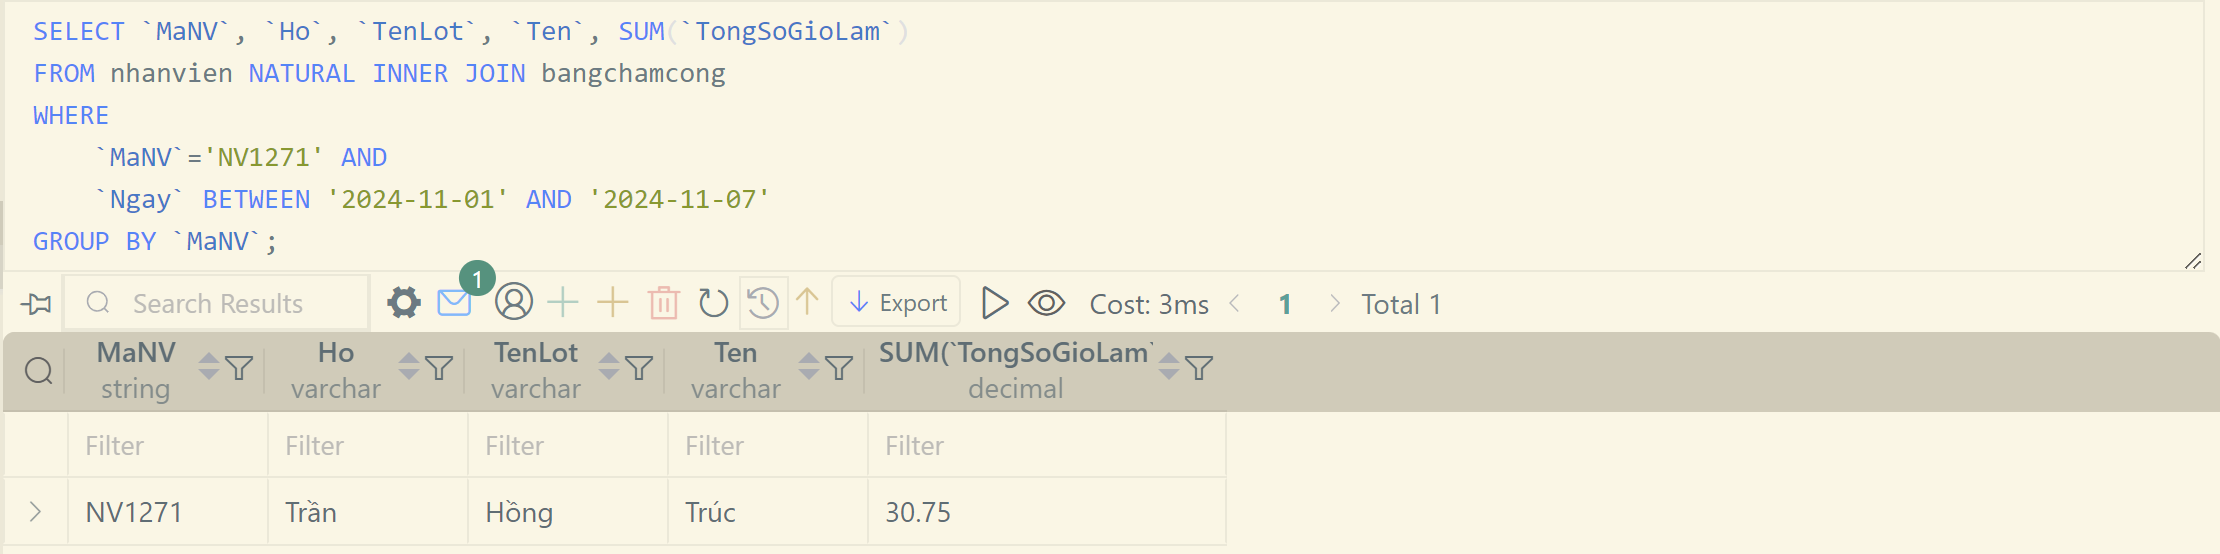
\includegraphics[width=\linewidth]{./content/images/extra_0.png}
        \caption{Kết quả câu lệnh tra cứu thông thường}
        \label{fig:extra_0}
    \end{figure}
    \item [--] Gọi hàm tonggiolamviec:
    \begin{figure}[H]
        \centering
        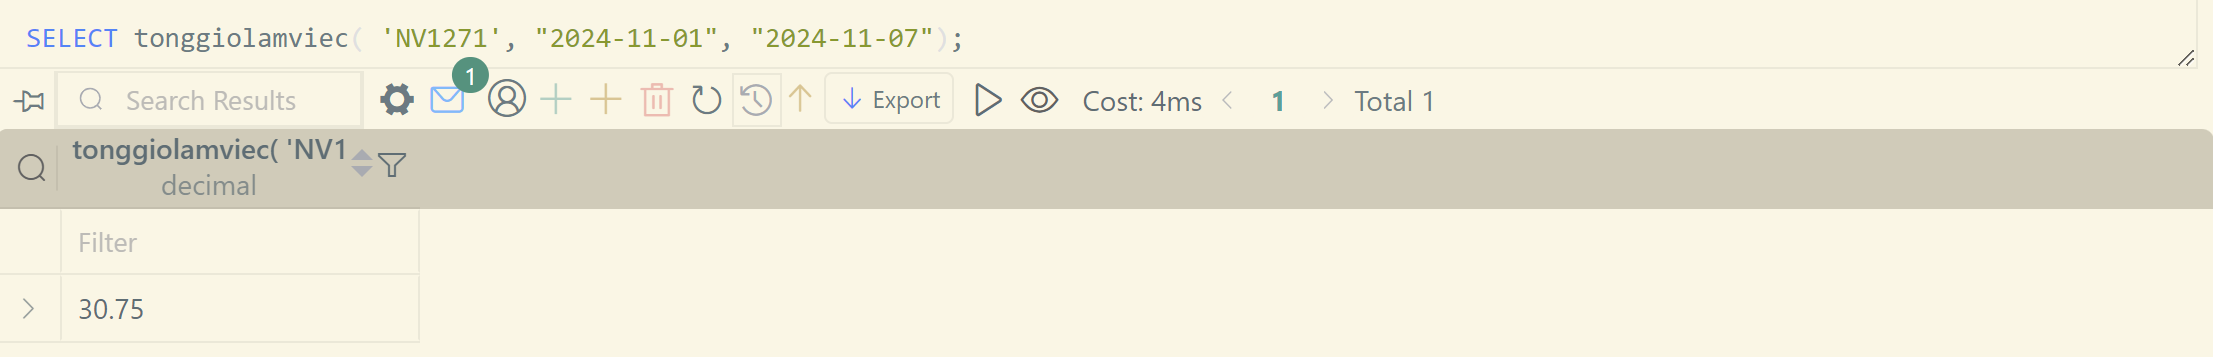
\includegraphics[width=\linewidth]{./content/images/extra_1.png}
        \caption{Kết quả câu lệnh gọi hàm tonggiolamviec}
        \label{fig:extra_1}
    \end{figure}
\end{itemize}

\newpage
\subsubsection{Procedure View\_Bangluong}
\textbf{Mô tả:} Thủ tục dùng để xem bảng lương trong khoảng thời gian xác định của các nhân viên trong một phòng ban cụ thể, hoặc toàn bộ nhân viên, có thể lọc theo loại nhân viên. Thủ tục này dùng để phục vụ việc hiển thị dữ liệu ở màn hình 3.

\textbf{input}:
\begin{itemize}
    \item [--] Tham số MaPhongBan, có kiểu \texttt{CHAR(6)}
    \item [--] Tham số EmpType, có kiểu \texttt{INT}
    \item [--] Tham số BeginDate, có kiểu \texttt{DATE}
    \item [--] Tham số EndDate, có kiểu \texttt{DATE}
\end{itemize}

\textbf{Output}: Bảng chứa thông tin của các nhân viên, số giờ làm việc trong quãng thời gian trên, lương tạm tính và lương thực tế của họ sau khi đã trừ đi thuế và bảo hiểm xã hội.

Câu lệnh khởi tạo thủ tục:
\begin{minted}{mysql}
    CREATE PROCEDURE View_BangLuong (MaPhongBan CHAR(6), EmpType INT, BeginDate DATE, EndDate DATE) 
    BEGIN
        DECLARE ThueSuat DECIMAL(5, 2);
        DECLARE BaoHiemXH DECIMAL(5, 2);
        
        SET ThueSuat = (SELECT bangthietlapluong.`ThueSuat` from bangthietlapluong WHERE `NgayApDung` <= EndDate ORDER BY `NgayApDung` DESC LIMIT 1);
        SET BaoHiemXH = (SELECT bangthietlapluong.`BaoHiemXH` from bangthietlapluong WHERE `NgayApDung` <= EndDate ORDER BY `NgayApDung` DESC LIMIT 1);
        
        IF EmpType = 0 THEN
            IF MaPhongBan = 'all' THEN 
                SELECT nhanvien.`MaNV`, CONCAT(nhanvien.`Ho`, ' ', nhanvien.`TenLot`, ' ', nhanvien.`Ten`) as TenNhanVien, tonggiolamviec(nhanvien.`MaNV`, BeginDate, EndDate) as TongGioLamViec, tinhluong(nhanvien.`MaNV`, BeginDate, EndDate) as LuongTamTinh, ((tinhluong(nhanvien.`MaNV`, BeginDate, EndDate) - tinhluong(nhanvien.`MaNV`, BeginDate, EndDate)*(BaoHiemXH))*(1 - ThueSuat)) as LuongThucTe FROM nhanvien;
            ELSE 
                SELECT nhanvien.`MaNV`, CONCAT(nhanvien.`Ho`, ' ', nhanvien.`TenLot`, ' ', nhanvien.`Ten`) as TenNhanVien, tonggiolamviec(nhanvien.`MaNV`, BeginDate, EndDate) as TongGioLamViec, tinhluong(nhanvien.`MaNV`, BeginDate, EndDate) as LuongTamTinh, ((tinhluong(nhanvien.`MaNV`, BeginDate, EndDate) - tinhluong(nhanvien.`MaNV`, BeginDate, EndDate)*(BaoHiemXH))*(1 - ThueSuat)) as LuongThucTe FROM nhanvien WHERE nhanvien.`MaPhongBan`=MaPhongBan;
            END IF;
\end{minted}
\begin{minted}[firstnumber=15]{mysql}
        ELSEIF EmpType = 1 THEN
            IF MaPhongBan = 'all' THEN 
                SELECT nhanvien.`MaNV`, CONCAT(nhanvien.`Ho`, ' ', nhanvien.`TenLot`, ' ', nhanvien.`Ten`) as TenNhanVien, tonggiolamviec(nhanvien.`MaNV`, BeginDate, EndDate) as TongGioLamViec, tinhluong(nhanvien.`MaNV`, BeginDate, EndDate) as LuongTamTinh, ((tinhluong(nhanvien.`MaNV`, BeginDate, EndDate) - tinhluong(nhanvien.`MaNV`, BeginDate, EndDate)*(BaoHiemXH))*(1 - ThueSuat)) as LuongThucTe FROM nhanvien NATURAL INNER JOIN nhanvientoanthoigian;
            ELSE 
                SELECT nhanvien.`MaNV`, CONCAT(nhanvien.`Ho`, ' ', nhanvien.`TenLot`, ' ', nhanvien.`Ten`) as TenNhanVien, tonggiolamviec(nhanvien.`MaNV`, BeginDate, EndDate) as TongGioLamViec, tinhluong(nhanvien.`MaNV`, BeginDate, EndDate) as LuongTamTinh, ((tinhluong(nhanvien.`MaNV`, BeginDate, EndDate) - tinhluong(nhanvien.`MaNV`, BeginDate, EndDate)*(BaoHiemXH))*(1 - ThueSuat)) as LuongThucTe FROM nhanvien NATURAL INNER JOIN nhanvientoanthoigian WHERE nhanvien.`MaPhongBan`=MaPhongBan;
            END IF;
        ELSEIF EmpType = -1 THEN
            IF MaPhongBan = 'all' THEN 
                SELECT nhanvien.`MaNV`, CONCAT(nhanvien.`Ho`, ' ', nhanvien.`TenLot`, ' ', nhanvien.`Ten`) as TenNhanVien, tonggiolamviec(nhanvien.`MaNV`, BeginDate, EndDate) as TongGioLamViec, tinhluong(nhanvien.`MaNV`, BeginDate, EndDate) as LuongTamTinh, ((tinhluong(nhanvien.`MaNV`, BeginDate, EndDate) - tinhluong(nhanvien.`MaNV`, BeginDate, EndDate)*(BaoHiemXH))*(1 - ThueSuat)) as LuongThucTe FROM nhanvien NATURAL INNER JOIN nhanvienbanthoigian;
            ELSE 
                SELECT nhanvien.`MaNV`, CONCAT(nhanvien.`Ho`, ' ', nhanvien.`TenLot`, ' ', nhanvien.`Ten`) as TenNhanVien, tonggiolamviec(nhanvien.`MaNV`, BeginDate, EndDate) as TongGioLamViec, tinhluong(nhanvien.`MaNV`, BeginDate, EndDate) as LuongTamTinh, ((tinhluong(nhanvien.`MaNV`, BeginDate, EndDate) - tinhluong(nhanvien.`MaNV`, BeginDate, EndDate)*(BaoHiemXH))*(1 - ThueSuat)) as LuongThucTe FROM nhanvien NATURAL INNER JOIN nhanvienbanthoigian WHERE nhanvien.`MaPhongBan`=MaPhongBan;
            END IF;
        END IF;
    END //
\end{minted}

\textbf{Thực thi thủ tục:} Xem bảng lương của các nhân viên thuộc phòng ban có mã phòng ban là 'PB0101' từ ngày 15/10/2024 đến ngày 31/10/2024, lần lượt lọc theo các loại nhân viên:
\begin{itemize}
    \item [--] Tất cả các nhân viên thuộc phòng ban 'PB0101'
    \begin{figure}[H]
        \centering
        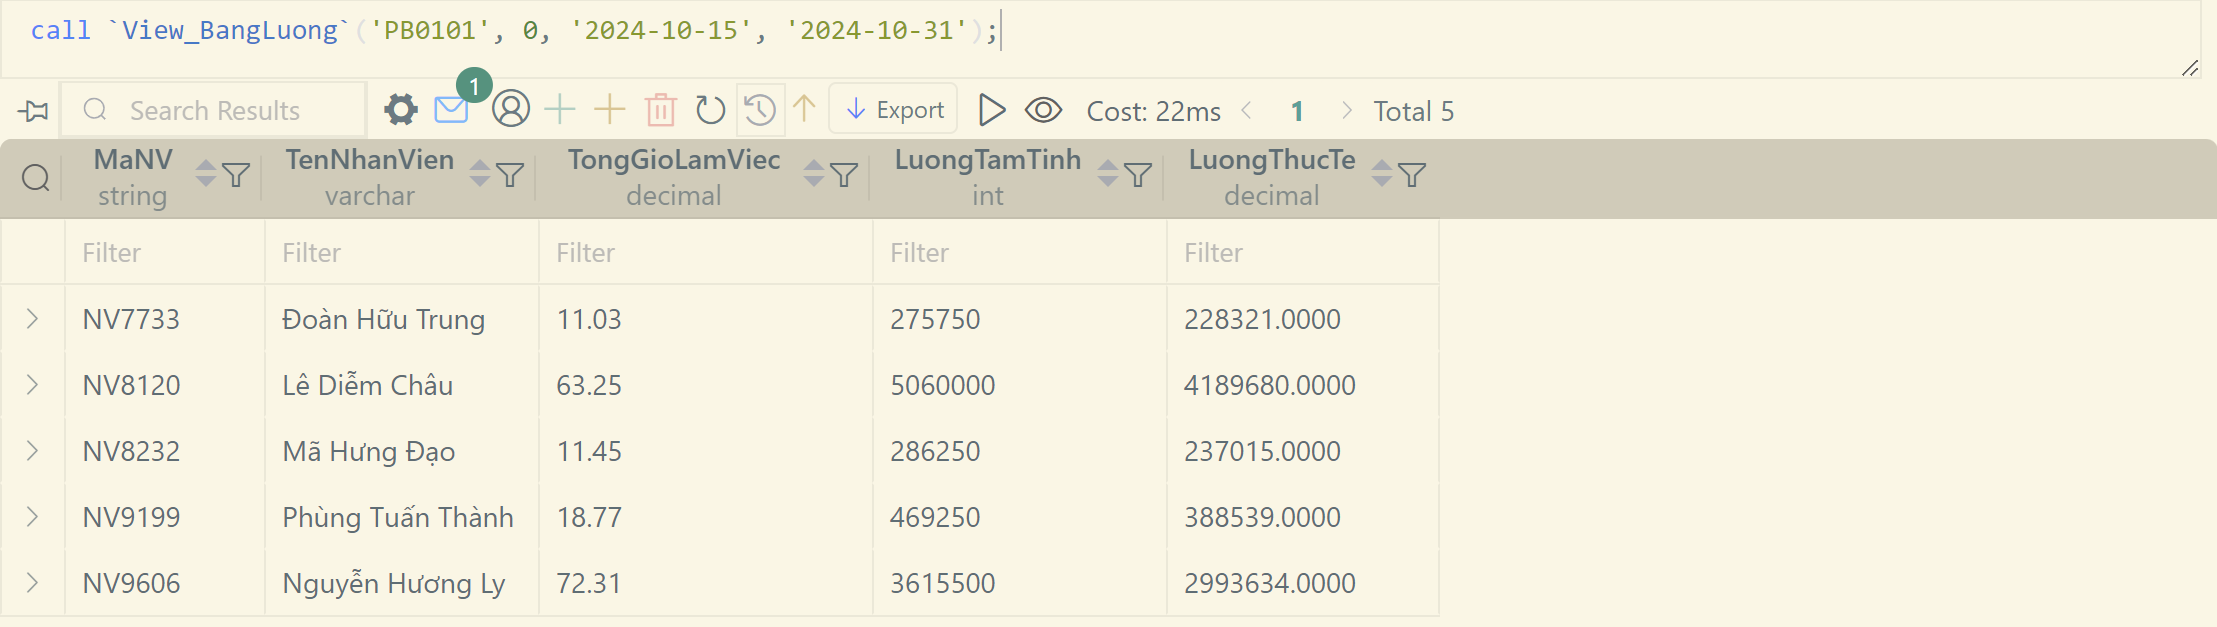
\includegraphics[width=\linewidth]{./content/images/extra_2.png}
        \caption{Bảng lương của tất cả các nhân viên thuộc phòng ban 'PB0101' từ ngày 15/10/2024 đến ngày 31/10/2024}
        \label{fig:extra_2}
    \end{figure}
    \item [--] Các nhân viên toàn thời gian thuộc phòng ban 'PB0101'
    \begin{figure}[H]
        \centering
        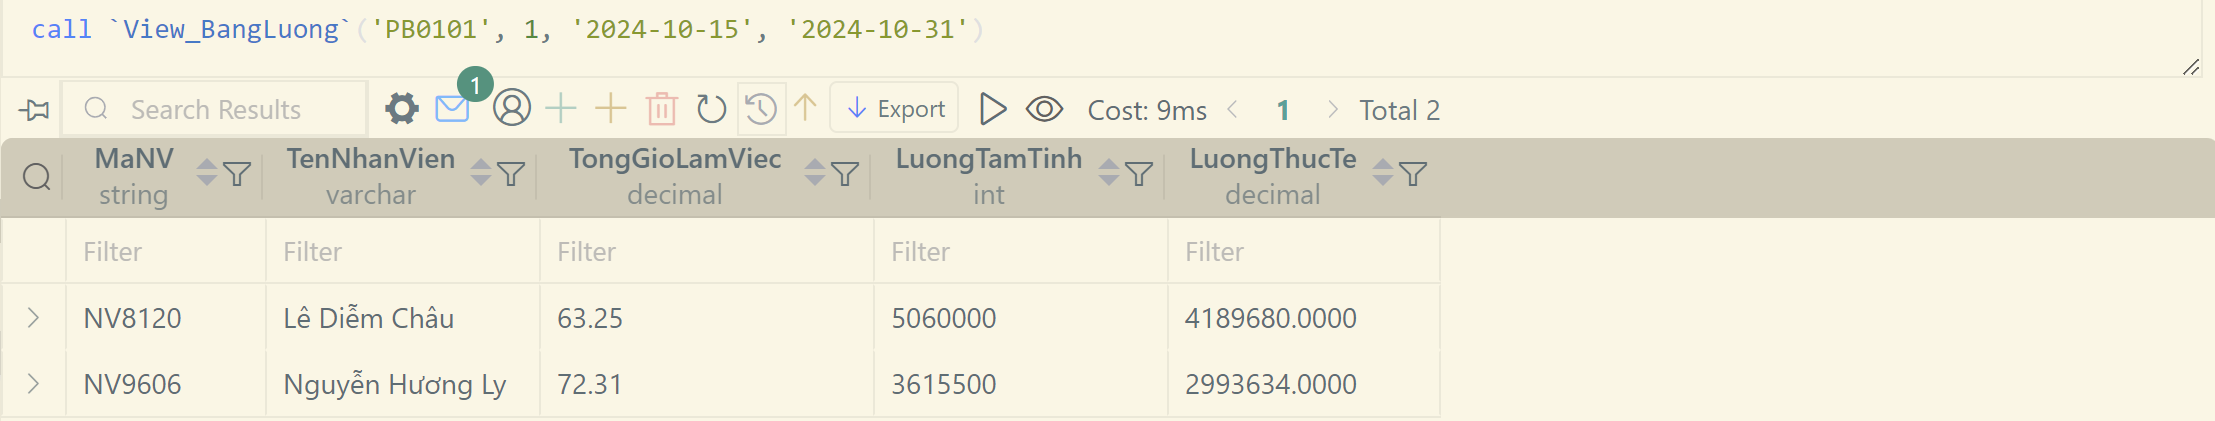
\includegraphics[width=\linewidth]{./content/images/extra_3.png}
        \caption{Bảng lương của các nhân viên toàn thời gian thuộc phòng ban 'PB0101' từ ngày 15/10/2024 đến ngày 31/10/2024}
        \label{fig:extra_3}
    \end{figure}
    \item [--] Các nhân viên bán thời gian thuộc phòng ban 'PB0101'
    \begin{figure}[H]
        \centering
        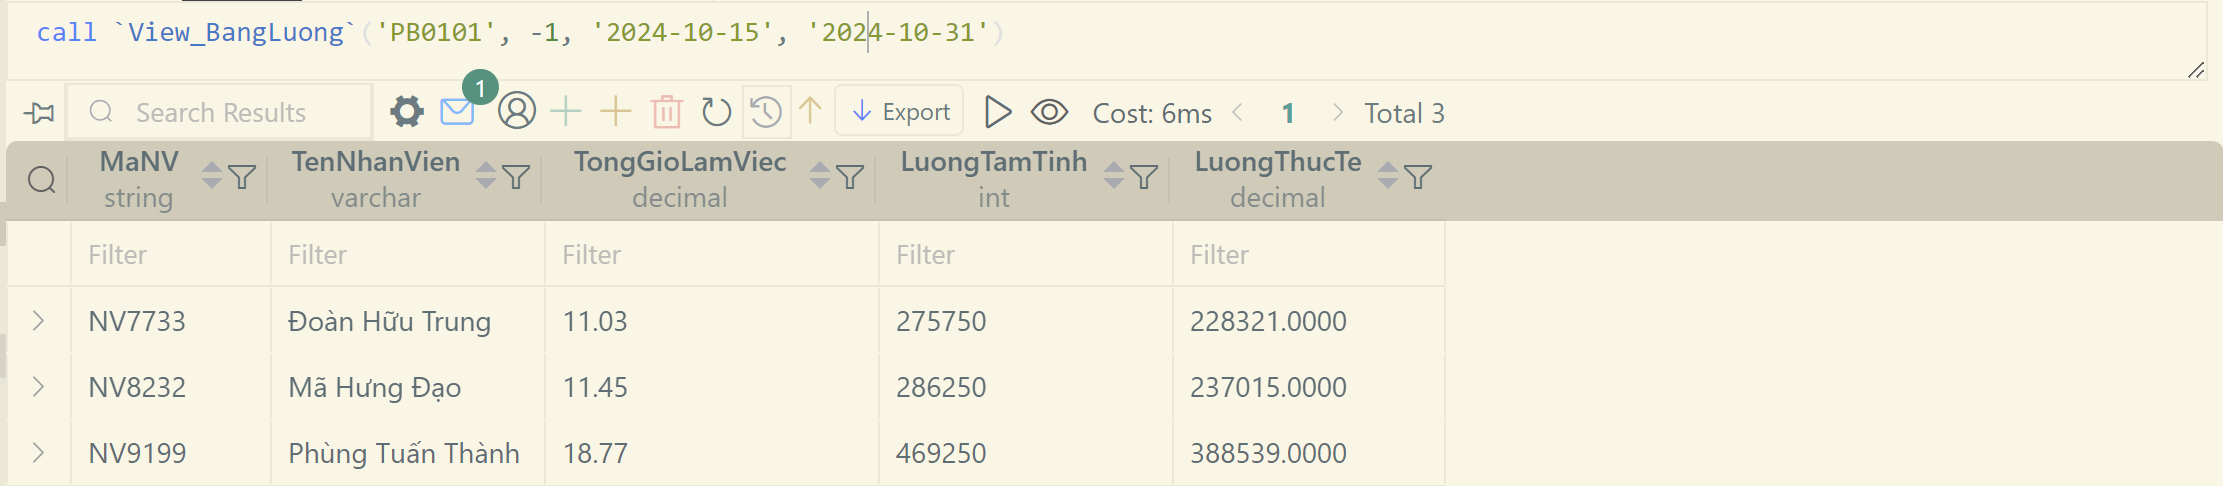
\includegraphics[width=\linewidth]{./content/images/extra_4.png}
        \caption{Bảng lương của các nhân viên bán thời gian thuộc phòng ban 'PB0101' từ ngày 15/10/2024 đến ngày 31/10/2024}
        \label{fig:extra_4}
    \end{figure}
\end{itemize}
\newpage